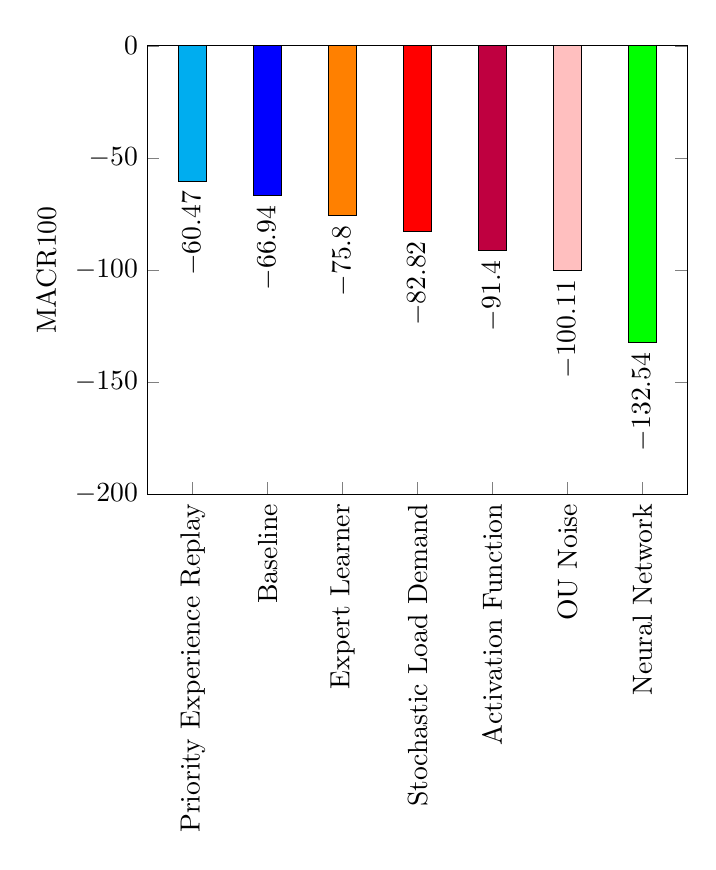
\begin{tikzpicture}
	\begin{axis}[
	    ylabel={MACR100},
	    symbolic x coords={Priority Experience Replay,, Baseline,, Expert Learner,, Stochastic Load Demand,, Activation Function,, OU Noise,, Neural Network},
	    xtick = {Baseline, Neural Network, Activation Function, OU Noise, Priority Experience Replay, Expert Learner, Stochastic Load Demand},
	    xticklabel style={rotate=90},
	    nodes near coords,
	    nodes near coords align={vertical},
	    every node near coord/.append style={rotate=90, anchor=east},
	    ymin=-200, ymax=0
	    ]
	\addplot [ybar, fill=blue] coordinates {(Baseline, -66.94)};
	\addplot [ybar, fill=green] coordinates {(Neural Network, -132.54)};
	\addplot [ybar, fill=purple] coordinates {(Activation Function, -91.40)};
	\addplot [ybar, fill=pink] coordinates {(OU Noise, -100.11)};
	\addplot [ybar, fill=cyan] coordinates {(Priority Experience Replay, -60.47)};
	\addplot [ybar, fill=orange] coordinates {(Expert Learner, -75.80)};
	\addplot [ybar, fill=red] coordinates {(Stochastic Load Demand, -82.82)};
	%\legend{Baseline, Neural Network, Activation Function, OU Noise, Priority Experience Replay, Expert Learner, Stochastic Load Demand};
	\end{axis}
\end{tikzpicture}